\PassOptionsToPackage{hyphens}{url}
\PassOptionsToPackage{usenames,dvipsnames,table}{xcolor}
\PassOptionsToPackage{breaklinks,colorlinks}{hyperref}
\documentclass[usenames, sigconf, 10pt]{acmart}

% conference specific style
\usepackage[]{natbib}

% common packages
\usepackage{silence}
\WarningFilter*{caption}{Unsupported document class}

\usepackage[hyphens]{url}
\urlstyle{same}
\usepackage[breaklinks,colorlinks]{hyperref}
\usepackage[usenames,dvipsnames]{xcolor}
\hypersetup{citecolor=RedOrange,linkcolor=NavyBlue,urlcolor=black}
\let\Bbbk\relax
\usepackage{amsmath,amsopn,amssymb}
%\usepackage{subfigure}
\usepackage{endnotes,microtype,xspace,graphicx,fancyvrb,multirow}
\usepackage{booktabs}
\usepackage{array,underscore,relsize}
\usepackage[T1]{fontenc}
%\usepackage{times}
%\usepackage{mathptmx}
\usepackage{fancyhdr}
\usepackage{enumitem}
\usepackage[labelfont=bf,font=small,skip=5pt]{caption}
\pagestyle{fancy}
\fancyhf{}
\renewcommand{\headrulewidth}{0pt}
\cfoot{\thepage}

% for math macro and numbers
\usepackage{fp}
\usepackage{siunitx}

% pseudo code
\usepackage{minted}

% balance bibliography
\usepackage{balance}

% use \num{123456} -> 123,456
\sisetup{group-separator={,},group-minimum-digits={3},output-decimal-marker={.}}

% comment environment
\usepackage{verbatim}

% listings
\usepackage{listings}
\usepackage{color}
\definecolor{lightgray}{rgb}{0.92, 0.92, 0.92}
\definecolor{lightgray1}{rgb}{0.82, 0.82, 0.82}
\definecolor{darkgray}{rgb}{0.4, 0.4, 0.4}
\definecolor{purple}{rgb}{0.65, 0.12, 0.82}
\definecolor{editorGray}{rgb}{0.95, 0.95, 0.95}
\definecolor{editorOcher}{rgb}{1, 0.5, 0} % #FF7F00 -> rgb(239, 169, 0)
\definecolor{editorGreen}{rgb}{0, 0.5, 0} % #007C00 -> rgb(0, 124, 0)
\definecolor{codegreen}{rgb}{0,0.6,0}
\definecolor{darkgreen}{rgb}{0,0.45,0}
\definecolor{codeblue}{rgb}{0,0,0.55}
\definecolor{linkblue}{rgb}{0,0,0.8}
\definecolor{darkred}{rgb}{0.8,0.1,0.15}
\definecolor{codegray}{rgb}{0.5,0.5,0.5}
\definecolor{codepurple}{rgb}{0.58,0,0.82}
\definecolor{backcolour}{rgb}{0.95,0.95,0.92}
\definecolor{mauve}{rgb}{0.58,0,0.82}

\lstset{
  language=PHP,                    % the language of the code
  alsolanguage=JAVA,
  alsolanguage=Python,
  alsolanguage=HTML,
  backgroundcolor=\color{white},   % choose the background color; you must add \usepackage{color} or \usepackage{xcolor}; should come as last argument
  basicstyle=\fontsize{7}{9}\ttfamily,        % the size of the fonts that are used for the code
  breakatwhitespace=false,         % sets if automatic breaks should only happen at whitespace
  breaklines=true,                 % sets automatic line breaking
  captionpos=b,                    % sets the caption-position to bottom
  commentstyle=\color{codegray},      % comment style
  deletekeywords={...},            % if you want to delete keywords from the given language
  escapeinside={\%*}{*)},          % if you want to add LaTeX within your code
  extendedchars=true,              % lets you use non-ASCII characters; for 8-bits encodings only, does not work with UTF-8
  frame=bt,	                   % adds a frame around the code
  keepspaces=true,                 % keeps spaces in text, useful for keeping indentation of code (possibly needs columns=flexible)
  keywordstyle=\color{darkgreen}\bfseries,       % keyword style
  ndkeywordstyle=\color{editorOcher}\ttfamily,
  morekeywords={*,...,string,=>,function,<?,php, NULL},            % if you want to add more keywords to the set
  numbers=left,                    % where to put the line-numbers; possible values are (none, left, right)
  numbersep=7pt,                   % how far the line-numbers are from the code
  numberstyle=\footnotesize\color{darkgray}\ttfamily, % the style that is used for the line-numbers
  rulecolor=\color{black},         % if not set, the frame-color may be changed on line-breaks within not-black text (e.g. comments (green here))
  showspaces=false,                % show spaces everywhere adding particular underscores; it overrides 'showstringspaces'
  showstringspaces=false,          % underline spaces within strings only
  showtabs=false,                  % show tabs within strings adding particular underscores
  stepnumber=1,                    % the step between two line-numbers. If it's 1, each line will be numbered
  stringstyle=\color{darkred}\ttfamily,        % string literal style
  tabsize=2,	                   % sets default tabsize to 2 spaces
  title=\lstname,                   % show the filename of files included with \lstinputlisting; also try caption instead of title
  firstnumber=1,
  identifierstyle=\color{codeblue},
  xleftmargin={2em},
  framexleftmargin={2em},
  %xrightmargin={6pt},
}

% algorithm
\usepackage[ruled, vlined, inoutnumbered, linesnumbered]{algorithm2e}



\newcommand{\sys}{\mbox{\textsc{NetPerfFuzz}}\xspace}

% ref. http://en.wikibooks.org/wiki/LaTeX/Colors
\newcommand{\PENGHUI}[1]{\textcolor{blue}{[PENGHUI: #1]}}
\newcommand{\XX}[0]{\textcolor{red}{XXX}}
\newcommand{\XXX}[1]{\textcolor{red}{XXX: #1}}
\newcommand{\TODO}[1]{\textcolor{Melon}{TODO: #1}}

\def\backtick{\char18}
\lstdefinestyle{mystyle}{literate={`}{\backtick}1, escapechar=@}

\usepackage{threeparttable}
\usepackage{caption}
\usepackage{subfig}
\newcommand{\blstinline}[1]{\lstinline[numbers=none, caption={}, frame={},stringstyle=\color{black}, deletekeywords={md5, foreach,strcmp, array, stripslashes},identifierstyle=\color{black},commentstyle=\color{black}]{#1}} % PENGHUI{I don't like the colors in inline code}
\renewcommand{\ttdefault}{pxtt}

%\newcommand{\URL}{\url}
\newcommand{\cc}[1]{\mbox{\smaller[0.5]\texttt{#1}}}

% enable the below for ACM camera ready
%\clubpenalty=10000
%\widowpenalty=10000
%\renewcommand*{\bibfont}{\raggedright}

%\linespread{1.2}

\fvset{fontsize=\scriptsize,xleftmargin=8pt,numbers=left,numbersep=5pt}


\makeatletter
\def\PY@reset{\let\PY@it=\relax \let\PY@bf=\relax%
    \let\PY@ul=\relax \let\PY@tc=\relax%
    \let\PY@bc=\relax \let\PY@ff=\relax}
\def\PY@tok#1{\csname PY@tok@#1\endcsname}
\def\PY@toks#1+{\ifx\relax#1\empty\else%
    \PY@tok{#1}\expandafter\PY@toks\fi}
\def\PY@do#1{\PY@bc{\PY@tc{\PY@ul{%
    \PY@it{\PY@bf{\PY@ff{#1}}}}}}}
\def\PY#1#2{\PY@reset\PY@toks#1+\relax+\PY@do{#2}}

\expandafter\def\csname PY@tok@w\endcsname{\def\PY@tc##1{\textcolor[rgb]{0.73,0.73,0.73}{##1}}}
\expandafter\def\csname PY@tok@c\endcsname{\let\PY@it=\textit\def\PY@tc##1{\textcolor[rgb]{0.25,0.50,0.50}{##1}}}
\expandafter\def\csname PY@tok@cp\endcsname{\def\PY@tc##1{\textcolor[rgb]{0.74,0.48,0.00}{##1}}}
\expandafter\def\csname PY@tok@k\endcsname{\let\PY@bf=\textbf\def\PY@tc##1{\textcolor[rgb]{0.00,0.50,0.00}{##1}}}
\expandafter\def\csname PY@tok@kp\endcsname{\def\PY@tc##1{\textcolor[rgb]{0.00,0.50,0.00}{##1}}}
\expandafter\def\csname PY@tok@kt\endcsname{\def\PY@tc##1{\textcolor[rgb]{0.69,0.00,0.25}{##1}}}
\expandafter\def\csname PY@tok@o\endcsname{\def\PY@tc##1{\textcolor[rgb]{0.40,0.40,0.40}{##1}}}
\expandafter\def\csname PY@tok@ow\endcsname{\let\PY@bf=\textbf\def\PY@tc##1{\textcolor[rgb]{0.67,0.13,1.00}{##1}}}
\expandafter\def\csname PY@tok@nb\endcsname{\def\PY@tc##1{\textcolor[rgb]{0.00,0.50,0.00}{##1}}}
\expandafter\def\csname PY@tok@nf\endcsname{\def\PY@tc##1{\textcolor[rgb]{0.00,0.00,1.00}{##1}}}
\expandafter\def\csname PY@tok@nc\endcsname{\let\PY@bf=\textbf\def\PY@tc##1{\textcolor[rgb]{0.00,0.00,1.00}{##1}}}
\expandafter\def\csname PY@tok@nn\endcsname{\let\PY@bf=\textbf\def\PY@tc##1{\textcolor[rgb]{0.00,0.00,1.00}{##1}}}
\expandafter\def\csname PY@tok@ne\endcsname{\let\PY@bf=\textbf\def\PY@tc##1{\textcolor[rgb]{0.82,0.25,0.23}{##1}}}
\expandafter\def\csname PY@tok@nv\endcsname{\def\PY@tc##1{\textcolor[rgb]{0.10,0.09,0.49}{##1}}}
\expandafter\def\csname PY@tok@no\endcsname{\def\PY@tc##1{\textcolor[rgb]{0.53,0.00,0.00}{##1}}}
\expandafter\def\csname PY@tok@nl\endcsname{\def\PY@tc##1{\textcolor[rgb]{0.63,0.63,0.00}{##1}}}
\expandafter\def\csname PY@tok@ni\endcsname{\let\PY@bf=\textbf\def\PY@tc##1{\textcolor[rgb]{0.60,0.60,0.60}{##1}}}
\expandafter\def\csname PY@tok@na\endcsname{\def\PY@tc##1{\textcolor[rgb]{0.49,0.56,0.16}{##1}}}
\expandafter\def\csname PY@tok@nt\endcsname{\let\PY@bf=\textbf\def\PY@tc##1{\textcolor[rgb]{0.00,0.50,0.00}{##1}}}
\expandafter\def\csname PY@tok@nd\endcsname{\def\PY@tc##1{\textcolor[rgb]{0.67,0.13,1.00}{##1}}}
\expandafter\def\csname PY@tok@s\endcsname{\def\PY@tc##1{\textcolor[rgb]{0.73,0.13,0.13}{##1}}}
\expandafter\def\csname PY@tok@sd\endcsname{\let\PY@it=\textit\def\PY@tc##1{\textcolor[rgb]{0.73,0.13,0.13}{##1}}}
\expandafter\def\csname PY@tok@si\endcsname{\let\PY@bf=\textbf\def\PY@tc##1{\textcolor[rgb]{0.73,0.40,0.53}{##1}}}
\expandafter\def\csname PY@tok@se\endcsname{\let\PY@bf=\textbf\def\PY@tc##1{\textcolor[rgb]{0.73,0.40,0.13}{##1}}}
\expandafter\def\csname PY@tok@sr\endcsname{\def\PY@tc##1{\textcolor[rgb]{0.73,0.40,0.53}{##1}}}
\expandafter\def\csname PY@tok@ss\endcsname{\def\PY@tc##1{\textcolor[rgb]{0.10,0.09,0.49}{##1}}}
\expandafter\def\csname PY@tok@sx\endcsname{\def\PY@tc##1{\textcolor[rgb]{0.00,0.50,0.00}{##1}}}
\expandafter\def\csname PY@tok@m\endcsname{\def\PY@tc##1{\textcolor[rgb]{0.40,0.40,0.40}{##1}}}
\expandafter\def\csname PY@tok@gh\endcsname{\let\PY@bf=\textbf\def\PY@tc##1{\textcolor[rgb]{0.00,0.00,0.50}{##1}}}
\expandafter\def\csname PY@tok@gu\endcsname{\let\PY@bf=\textbf\def\PY@tc##1{\textcolor[rgb]{0.50,0.00,0.50}{##1}}}
\expandafter\def\csname PY@tok@gd\endcsname{\def\PY@tc##1{\textcolor[rgb]{0.63,0.00,0.00}{##1}}}
\expandafter\def\csname PY@tok@gi\endcsname{\def\PY@tc##1{\textcolor[rgb]{0.00,0.63,0.00}{##1}}}
\expandafter\def\csname PY@tok@gr\endcsname{\def\PY@tc##1{\textcolor[rgb]{1.00,0.00,0.00}{##1}}}
\expandafter\def\csname PY@tok@ge\endcsname{\let\PY@it=\textit}
\expandafter\def\csname PY@tok@gs\endcsname{\let\PY@bf=\textbf}
\expandafter\def\csname PY@tok@gp\endcsname{\let\PY@bf=\textbf\def\PY@tc##1{\textcolor[rgb]{0.00,0.00,0.50}{##1}}}
\expandafter\def\csname PY@tok@go\endcsname{\def\PY@tc##1{\textcolor[rgb]{0.53,0.53,0.53}{##1}}}
\expandafter\def\csname PY@tok@gt\endcsname{\def\PY@tc##1{\textcolor[rgb]{0.00,0.27,0.87}{##1}}}
\expandafter\def\csname PY@tok@err\endcsname{\def\PY@bc##1{\setlength{\fboxsep}{0pt}\fcolorbox[rgb]{1.00,0.00,0.00}{1,1,1}{\strut ##1}}}
\expandafter\def\csname PY@tok@kc\endcsname{\let\PY@bf=\textbf\def\PY@tc##1{\textcolor[rgb]{0.00,0.50,0.00}{##1}}}
\expandafter\def\csname PY@tok@kd\endcsname{\let\PY@bf=\textbf\def\PY@tc##1{\textcolor[rgb]{0.00,0.50,0.00}{##1}}}
\expandafter\def\csname PY@tok@kn\endcsname{\let\PY@bf=\textbf\def\PY@tc##1{\textcolor[rgb]{0.00,0.50,0.00}{##1}}}
\expandafter\def\csname PY@tok@kr\endcsname{\let\PY@bf=\textbf\def\PY@tc##1{\textcolor[rgb]{0.00,0.50,0.00}{##1}}}
\expandafter\def\csname PY@tok@bp\endcsname{\def\PY@tc##1{\textcolor[rgb]{0.00,0.50,0.00}{##1}}}
\expandafter\def\csname PY@tok@fm\endcsname{\def\PY@tc##1{\textcolor[rgb]{0.00,0.00,1.00}{##1}}}
\expandafter\def\csname PY@tok@vc\endcsname{\def\PY@tc##1{\textcolor[rgb]{0.10,0.09,0.49}{##1}}}
\expandafter\def\csname PY@tok@vg\endcsname{\def\PY@tc##1{\textcolor[rgb]{0.10,0.09,0.49}{##1}}}
\expandafter\def\csname PY@tok@vi\endcsname{\def\PY@tc##1{\textcolor[rgb]{0.10,0.09,0.49}{##1}}}
\expandafter\def\csname PY@tok@vm\endcsname{\def\PY@tc##1{\textcolor[rgb]{0.10,0.09,0.49}{##1}}}
\expandafter\def\csname PY@tok@sa\endcsname{\def\PY@tc##1{\textcolor[rgb]{0.73,0.13,0.13}{##1}}}
\expandafter\def\csname PY@tok@sb\endcsname{\def\PY@tc##1{\textcolor[rgb]{0.73,0.13,0.13}{##1}}}
\expandafter\def\csname PY@tok@sc\endcsname{\def\PY@tc##1{\textcolor[rgb]{0.73,0.13,0.13}{##1}}}
\expandafter\def\csname PY@tok@dl\endcsname{\def\PY@tc##1{\textcolor[rgb]{0.73,0.13,0.13}{##1}}}
\expandafter\def\csname PY@tok@s2\endcsname{\def\PY@tc##1{\textcolor[rgb]{0.73,0.13,0.13}{##1}}}
\expandafter\def\csname PY@tok@sh\endcsname{\def\PY@tc##1{\textcolor[rgb]{0.73,0.13,0.13}{##1}}}
\expandafter\def\csname PY@tok@s1\endcsname{\def\PY@tc##1{\textcolor[rgb]{0.73,0.13,0.13}{##1}}}
\expandafter\def\csname PY@tok@mb\endcsname{\def\PY@tc##1{\textcolor[rgb]{0.40,0.40,0.40}{##1}}}
\expandafter\def\csname PY@tok@mf\endcsname{\def\PY@tc##1{\textcolor[rgb]{0.40,0.40,0.40}{##1}}}
\expandafter\def\csname PY@tok@mh\endcsname{\def\PY@tc##1{\textcolor[rgb]{0.40,0.40,0.40}{##1}}}
\expandafter\def\csname PY@tok@mi\endcsname{\def\PY@tc##1{\textcolor[rgb]{0.40,0.40,0.40}{##1}}}
\expandafter\def\csname PY@tok@il\endcsname{\def\PY@tc##1{\textcolor[rgb]{0.40,0.40,0.40}{##1}}}
\expandafter\def\csname PY@tok@mo\endcsname{\def\PY@tc##1{\textcolor[rgb]{0.40,0.40,0.40}{##1}}}
\expandafter\def\csname PY@tok@ch\endcsname{\let\PY@it=\textit\def\PY@tc##1{\textcolor[rgb]{0.25,0.50,0.50}{##1}}}
\expandafter\def\csname PY@tok@cm\endcsname{\let\PY@it=\textit\def\PY@tc##1{\textcolor[rgb]{0.25,0.50,0.50}{##1}}}
\expandafter\def\csname PY@tok@cpf\endcsname{\let\PY@it=\textit\def\PY@tc##1{\textcolor[rgb]{0.25,0.50,0.50}{##1}}}
\expandafter\def\csname PY@tok@c1\endcsname{\let\PY@it=\textit\def\PY@tc##1{\textcolor[rgb]{0.25,0.50,0.50}{##1}}}
\expandafter\def\csname PY@tok@cs\endcsname{\let\PY@it=\textit\def\PY@tc##1{\textcolor[rgb]{0.25,0.50,0.50}{##1}}}

\def\PYZbs{\char`\\}
\def\PYZus{\char`\_}
\def\PYZob{\char`\{}
\def\PYZcb{\char`\}}
\def\PYZca{\char`\^}
\def\PYZam{\char`\&}
\def\PYZlt{\char`\<}
\def\PYZgt{\char`\>}
\def\PYZsh{\char`\#}
\def\PYZpc{\char`\%}
\def\PYZdl{\char`\$}
\def\PYZhy{\char`\-}
\def\PYZsq{\char`\'}
\def\PYZdq{\char`\"}
\def\PYZti{\char`\~}
% for compatibility with earlier versions
\def\PYZat{@}
\def\PYZlb{[}
\def\PYZrb{]}
\makeatother


\newcommand{\figrule}{\hrule width \hsize height .33pt}
\newcommand{\coderule}{\vspace{-0.5em}\figrule\vspace{0.2em}}

\setlength{\abovedisplayskip}{0pt}
\setlength{\abovedisplayshortskip}{0pt}
\setlength{\belowdisplayskip}{0pt}
\setlength{\belowdisplayshortskip}{0pt}
\setlength{\jot}{0pt}

\def\Snospace~{\S{}}
\renewcommand*\sectionautorefname{\Snospace}
\def\sectionautorefname{\Snospace}
\def\subsectionautorefname{\Snospace}
\def\subsubsectionautorefname{\Snospace}
\def\chapterautorefname{\Snospace}
%\renewcommand{\figurename}{Fig.}
%\def\figureautorefname{\figurename}
\renewcommand{\algorithmautorefname}{Algorithm}
\newcommand*{\Appendixautorefname}{Appendix}
\newcommand{\subfigureautorefname}{\figureautorefname}

%\numberwithin{equation}{section}
\newcommand{\yes}{Y}
\newcommand{\no}{}

% sema
\newcommand{\shl}{\ \cc{<}\cc{<}\ }
\newcommand{\shr}{\ \cc{>}\cc{>}\ }
\newcommand{\x}{$\times$\xspace}

\if 0
\renewcommand{\topfraction}{0.9}
\renewcommand{\dbltopfraction}{0.9}
\renewcommand{\bottomfraction}{0.8}
\renewcommand{\textfraction}{0.05}
\renewcommand{\floatpagefraction}{0.9}
\renewcommand{\dblfloatpagefraction}{0.9}
\setcounter{topnumber}{10}
\setcounter{bottomnumber}{10}
\setcounter{totalnumber}{10}
\setcounter{dbltopnumber}{10}
\fi

\newif\ifdraft\drafttrue
\newif\ifnotes\notestrue
\ifdraft\else\notesfalse\fi

\newcommand{\eg}{{\em e.g.}}
\newcommand{\etal}{{\em et al.}}
\newcommand{\etc}{{\em etc.}}
\newcommand{\ie}{{\em i.e.}}

% hide comments
% \renewcommand{\TK}[1]{\ignorespaces}
% \renewcommand{\XXX}[1]{\ignorespaces}
% \renewcommand{\TODO}[1]{\ignorespaces}
% \renewcommand{\YINXI}[1]{\ignorespaces}
% \renewcommand{\PENGHUI}[1]{\ignorespaces}

%% Ensure ligatures (e.g., ``fine official flag'') can be copy/pasted from PDF.
\input{glyphtounicode}
\pdfgentounicode=1

\newcolumntype{R}[1]{>{\raggedleft\let\newline\\\arraybackslash\hspace{0pt}}p{#1}}

% include macros
\newcommand{\includepdf}[1]{
  \includegraphics[width=\columnwidth]{#1}
}
\newcommand{\includeplot}[1]{
  \resizebox{\columnwidth}{!}{\input{#1}}
}

% list
\newcommand{\squishlist}{
\begin{itemize}[noitemsep,nolistsep]
  \setlength{\itemsep}{-0pt}
}
\newcommand{\squishend}{
  \end{itemize}
}

%%
%% NOTE.
%%  to use circled number in caption, use
%%   (e.g., \protect\WC{1})
%%
\usepackage{tikz}
\newcommand*\WC[1]{%
\begin{tikzpicture}[baseline=(C.base)]
\node[draw,circle,inner sep=0.2pt](C) {#1};
\end{tikzpicture}}

\newcommand*\BC[1]{%
\begin{tikzpicture}[baseline=(C.base)]
\node[draw,circle,fill=black,inner sep=0.2pt](C) {\textcolor{white}{#1}};
\end{tikzpicture}}

\usepackage{xstring}
\newcommand{\PP}[1]{
\vspace{2px}
\noindent{\bf \IfEndWith{#1}{.}{#1}{#1.}}
}

\newcommand{\PN}[1]{
\vspace{2px}
\noindent{\bf #1}
}

\newcommand{\ra}[1]{\renewcommand{\arraystretch}{#1}}
\newcommand{\V}{\checkmark}
\newcommand{\X}{{\footnotesize $\times$}\xspace}
\renewcommand{\O}{\phantom{0}}

%% units
\newcommand{\B}{\,\text{B}\xspace}
\newcommand{\K}{\,\text{K}\xspace}
\newcommand{\M}{\,\text{M}\xspace}
\newcommand{\T}{\,\text{T}\xspace}
\newcommand{\KB}{\,\text{KB}\xspace}
\newcommand{\MB}{\,\text{MB}\xspace}
\newcommand{\GB}{\,\text{GB}\xspace}
\newcommand{\TB}{\,\text{TB}\xspace}

\newcommand{\Bs}{\,\text{B/s}\xspace}
\newcommand{\KBs}{\,\text{KB/s}\xspace}
\newcommand{\MBs}{\,\text{MB/s}\xspace}
\newcommand{\GBs}{\,\text{GB/s}\xspace}

% boxbeg/end
\newcommand{\boxbeg}{
\vspace{2px}
\noindent\begin{tabular}{|l|}\hline
\begin{minipage}{3.2in}
\vspace{2px}
\noindent
}

\newcommand{\boxend}{
\vspace{2px}
\end{minipage}\\ \hline
\end{tabular}
\vspace{-10pt}
}

\gdef\therev{4275d75}
\gdef\thedate{2021-04-16 19:48:04 +0800}

\renewcommand\thefootnote{\textcolor{blue}{\arabic{footnote}}}

%\setcopyright{iw3c2w3}
\usepackage[toc]{appendix}
%-------------------------------------------------------------------------------
\usepackage{diagbox}
\begin{document}
%-------------------------------------------------------------------------------

\title[]{Understanding and Detecting Bugs in Network Operating Systems}

\author{Penghui Li 1155137827}
\email{phli@cse.cuhk.edu.hk}
\settopmatter{printacmref=false, printccs=false, printfolios=false}
\setcopyright{none}
%\setcopyright{iw3c2w3}
\copyrightyear{2021}
\acmYear{2021}
\acmConference[CSCI '5570]{Large Scale Data Processing Systems}{Spring 2021}{CUHK}
\acmBooktitle{Large Scale Data Processing Systems}
\acmPrice{}
\acmDOI{}
\acmISBN{}




\begin{abstract}
Network systems connect the Internet world.
Bugs in network systems can lead to denial-of-service, performance issues, \etc{}
Understanding network system bugs can benefit both the system developers and security analysts.

However, to the best of our knowledge, the bugs in network systems have not been well understood. 
    The potential security impact has not been well investigated as well.
    In this project, we aim to understand the bugs in network systems. 
    We hope to learn lessons to further guide future bug detection in network systems.
\end{abstract}

%\date{}
\maketitle

\sloppy

\section{Introduction}
\label{s:intro}
Network Operating Systems (NOSs) connect multiple computers and devices and manage network resources in the settings of Software Defined Networking (SDN).
%
NOSs manage multiple requests concurrently and provide the security in multiuser environments. 
%
To date, there are many NOSs being proposed and matained by network service vendors.
%
For example, Cisco Internetwork Operating System is a family of network operating systems used on many Cisco Systems routers and current Cisco network switches \cite{edgeworth2014ip};
DD-WRT \cite{dd-wrt} is a Linux based open-sourced NOS suitable for various WLAN routers and embedded systems.
%
%

Due to their popularity and critical uses, the bugs in these network operating systems can lead to severe security consequences.
%
In particular, network operating systems could have performance bugs, which cause excessive resource consumption and could negatively affect user experiences.
%
They can be further leveraged by attackers for launching application-layer denial-of-service (DoS) attacks \cite{crosby2003algodos}.
%
By specially crafting inputs to trigger a performance bug in the network operating systems,
%
the attacker can exhaust the server's resources (\eg{,} memory and CPU) and make the services unavailable to normal users. 

%
To the best of our knowledge, there currently has little knowledge about the prevalence of performance bugs in the wild.
%performance bugs.
%
Prior studies on compilers generally focus on memory corruptions,
%
whereas performance bugs, especially in close-sourced network operating systems, are not well investigated and understood yet.
%
Some works studied performance issues in the regular expression engines \cite{shen2018rescue,wustholz2017static}, desktop software \cite{perfbugstudy}, and Android applications \cite{liu2014characterizing}.
%
Network operating systems, however, have not been covered.
%
To this end, we conduct a comprehensive study of the performance bugs in network operating systems to answer the following research questions:
%
\begin{itemize}[itemsep=0.5ex, parsep=0ex, leftmargin=3mm]
    \item What are the main categories of the bugs?
    \item What are the main factors that cause bugs?
    \item How widespread are the bugs in network operating systems?
    \item How severe are the bugs in network operating systems?
\end{itemize}

We empirically analyze \XX known performance bugs in mainstream network operating systems and thoroughly summarize their characteristics.
%
We observe that there has been a continuous growth in the number of reported performance bugs in the past 3 years.
%
We further identify that the ways that network operating systems handle the language's context-sensitive features are the dominant root cause of the performance bugs.
%
We reveal that the developers of network operating systems usually mitigate such exploitation by enforcing a hard limit for the maximum number of backtracking for certain tasks, which, however, limits the intended functionality of the network operating systems.


In this work, we also explore detecting performance bugs in network operating systems.
%
To the best of our knowledge, there is not any tailored tools specially designed for detecting performance bugs in network operating systems.
%
Fuzzing \cite{slowfuzz, hotfuzz, perffuzz} eliminates the limitations of static analysis techniques 
(\eg{,} high false positives) 
\cite{perfbugstudy, nistor2013toddler,nistor2015caramel}.
%
It has become the go-to approach with thousands of vulnerabilities in real-world software.
%
Without a doubt, performance bugs in network operating systems can be fuzzed as well.
%
%However, existing fuzzers \cite{slowfuzz, perffuzz} for performance bugs are not aware of special \emph{contex} of network operating systems and cannot effectively generate inputs to thoroughly exercise them.
%
%Therefore, besides the bit/byte level mutation \cite{afl}, we summarize the rules of the inputs. 
%
%We develop a syntax-tree based mutation strategy \cite{superion} to preserve and extend useful rules during the input mutation.
%
%This helps to generate inputs more effectively.
%
%

We mainly focus on CPU exhaustion performance bugs.
%
To detect them, we monitor the program execution under the generated inputs.
%
We employ a statistical model using Chebyshev inequality to label abnormal cases as performance bugs.
%
This can potentially cause duplicate bug reports as multiple bug reports with only slight difference in the inputs actually trigger the same bug.
%
It is time-consuming and impractical to leverage human efforts to manually de-duplicate them.
%
Existing bug de-duplicating methods using coverage profile and call stacks are inaccurate and not applicable to performance bugs.
%
For example, it is hard to obtain an accurate and deterministic call stack that reveals the situation when a performance bug is triggered.
%
Therefore, we propose a execution trace similarity comparison algorithm to de-duplicate the reports.
%
Specifically, we represent the execution trace of each report into a vector;
%
we compute the cosine similarity between vector pairs and classify vectors (bug reports) with high similarity as the same bug.
%

We integrate abovementioned techniques into \sys.
%
We demonstrated \sys outperformed the state-of-the-art works \cite{slowfuzz, perffuzz} \emph{better} performance slowdown, and \emph{higher} code coverage.
\sys is highly effective in generating test cases to trigger new code in the testing network operating systems.
%
Though we have not identified any new bugs yet after 6-hour testing, we plan to further keep \sys running for more time.
%
Hopenfully, our techniques can help find new bugs in the future.

In summary, we make the following contributions in this work.
\begin{itemize}
    \item
        We conduct a systematic study on performance bugs in network operating systems.
        %
        We present an empirical understanding of the performance bugs and the patches.
        %
    \item We develop a new system, \sys, to effectively generate useful inputs to detect performance bugs in network operating systems.
        %
    \item We demonstrate \sys can significantly outperform the state-of-the-art works.
\end{itemize}

\section{Background}
\label{s:background}

\subsection{Performance Bugs}
\label{s:background-bug}
%\TODO{Have not had time to rephrase the decriptions from 'parser'->'compiler'}
Performance bugs in a program could degrade its performance and waste computational resources.
%
Usually, people define performance bugs as software defects where relatively simple \emph{source-code} changes can significantly optimize the execution of the software while preserving the functionality \cite{perfbugstudy, killian2010finding, s2e}.
%
There can be several different performance issues regarding different categories of resources.
%
For example, some performance bugs could cause excessive CPU resource utilization, resulting in unexpectedly longer execution time; 
%
some other bugs could lead to huge memory consumption because of uncontrolled memory allocation and memory leak \cite{wen2020memlock}.
%

%they 
Performance bugs lead to reduced throughput, increased latency, and wasted resources in software.
%
They particularly impact the end-user experiences.
%
What is worse, when a buggy application is deployed on the web servers, the bugs can be exploited by attackers for denial-of-service attacks, which can impair the availability of the services \cite{rampart}.
%
In the past, performance bugs have caused several publicized failures, causing many software projects to be abandoned \cite{perfbugstudy, lessons}.

\subsection{Network Operating Systems}
\label{s:background-nos}
Network operating system is a computer operating system that facilitates to connect and communicate various autonomous computers over a network. 
%
An autonomous computer is an independent computer that has its own local memory, hardware, \etc{}
%
It is self capable to perform operations and processing for a single user. 
%
Network operating systems can be embedded in a router or hardware firewall that operates the functions in the network layer \cite{al2001dialoguer}.
%
Typical real-world network operating systems include Cisco IOS \cite{cisco-ios}, DD_WRT \cite{dd-wrt}, Cumulus Linux \cite{cumulus-linux}, \etc{}



%\input{problem}
\section{Understanding Performance Bugs} 
\label{s:study}
%To the best of our knowledge, there is currently little knowledge about 
%
In this section, we present an empirical study on several known performance bugs in mainstream network operating systems 
to help understand their characteristics. % of the performance bugs. % in Markdown compilers.
%

\subsection{Data Collection}
\label{s:study-bug}

\iffalse
\begin{table}[t]
\centering
    \caption{The existing performance bugs included in our study.
    %Lang. means the underlying programming language for implementing the Markdown compiler.
    }
\label{table:study-dataset}
\small
%\resizebox{0.47\textwidth}{!}{
\begin{tabular}{lcc}
   \toprule
      Software  & \# Bugs & Time Periods \\
    \midrule
    Cicso IOS \cite{cicso-ios} & 58 & 10/26/2001 - 01/13/2021 \\
     & & 01/14/2017 - 12/20/2020 \\
    MD4C & 6 & 03/10/2019 - 09/10/2019\\
    commonmark.js & 9 & 09/28/2017 - 08/13/2019 \\
    markdown-it & 8 & 08/14/2019 - 11/20/2020\\
%    \midrule
%    Total &  & (49) 52 & 10/26/2014 - 12/20/2020\\
   \bottomrule
\end{tabular}
%}
\end{table}
\fi

%As shown in \autoref{table:study-dataset}, 
%
We investigate performance bugs in the Cicso IOS \cite{cicso-ios}, 
%
which is one of the most popular network operating systems.
%
Ideally, if more network operating systems are included in the study we can present a more comprehensive characteriazation.
%
However, due the the limited time and human labours allowed for this work,
%
we have to somehow restrict the study scope.
%
Nevertheless, this work, as an early stage studying performance bugs in network operating systems, shall provide some general inspirations for future network system security analysis.

We manually collected 58 distinct performance bugs from the database of Common Vulenrabilities and Exposures (CVE) \cite{cve}.
%
The detailed information about the vulnerabilities included in our study is presented in \autoref{cve-details}.
%
Some bug reports might be duplicates.
%
We remove a duplicate bug from our dataset if it has a similar cause as another one,
%
though it can have a different exploit vector.
%
In summary, we obtained 49 distinct performance bugs by removing \XXX duplicates from the ones reported from November 2001 to January 2021.
%
We found all these performance bugs were abusing the CPU resources or memory resources.
%
%This suggests CPU resource exhaustion performance bugs are the dominant type of performance bugs.

We next characterize the performance bugs and present our findings.

\subsection{Bug Disclosure Over Time}
\label{s:study-time}

\begin{figure}[t]
    \centering
    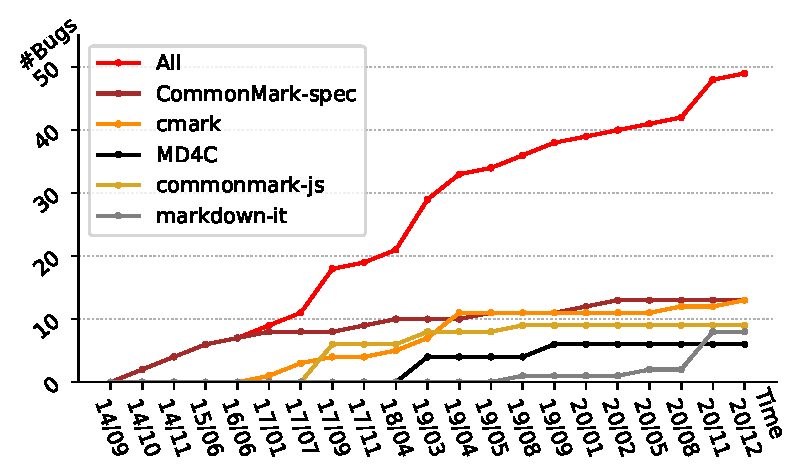
\includegraphics[width=0.45\textwidth, trim =5 0 0 0,clip]{fig/disclosure-time.pdf}
    \caption{The number of performance bug reports over time.
    }
    \label{fig:disclosure-time}
\end{figure}

To understand the trend of performance bugs, we analyze the disclosure time of them.  
We depict the number of performance bugs along the time they were disclosed in \autoref{fig:disclosure-time}.
%
We observe that few bugs were reported before early 2004, and the number of reported bugs had been gradually growing from early 2018 till late 2020.
%
In particular, 28 (57.14\%) out of the 49 performance bugs were disclosed from April 2018 till December 2020 (22 months);
%
21 (42.86\%) bugs were reported from August 2014 to December 2017 (41 months).
%
It reveals that such bugs had been gradually drawing the attention from the compiler developers and security analysts.
%

\subsection{Root Causes}
\label{s:study-root-causes}
%
Identifying the common root causes of real-world performance bugs can benefit potential future research and software developments.
%
We manually analyzed the performance bugs and successfully figured out the root causes for \XX bugs.
%
We classify the root causes into three categories.
%
A bug is assigned to multiple categories if it has multiple major causes.


\PN{R1:} \emph{Super-linear algorithms.}
Some normal algorithms implemented in Markdown compilers have super-linear worst-case complexity \cite{slowfuzz, perffuzz}.
%
Attackers can craft inputs to trigger the worst-case behaviors and lead to performance issues.
%
%For instance, some compilers use regular expressions to match inputs, which are vulnerable to ReDoS attacks \cite{redos} that trigger excessive numbers of backtracking in the matching process.
%
The majority (25 out of 39) of bugs were related to such worst-case behaviors.
%\WM{Check this number again after moving ReDoS to R2.}
%
%Specifically, the abnormal backtracking logic in Markdown compilers can be further divided into two groups:
%
%
%Known performance bugs in this category exploit either the design of Markdown compilers or the vulnerable regular expression and can lead to polynomial or exponential complexity compilation time.
%
%What is worse, the intended normal functionality of the Markdown compilers can be abused by crafted inputs for triggering worst-case behaviors, \eg{,} excessive number of backtracking.
%
%This includes triggering cataphoric backtracking in regular expression matches and the similar logic design inside the Markdown compilers can be abused with specially crafted inputs.
%
%
%If the input size is not limited, the Markdown compilers can easily hang for up to several hours.
%
%
%27 out of 39 performance bugs belong to this category.
%Specially crafted inputs abuse the backtracking behaviors and lead.
%
%We investigate the specially crafted inputs that lead to such worst-case behaviors. %and present two bugs in this category.
%We discuss two primary kinds of algorithms that exhibit the super-linear worst-case complexity we find. % in the Markdown compilers.
%
%They can be roughly divided into two groups:
%
%(1) long open tokens without close tokens,
%
%and (2) long early open tokens and late close tokens.
%

Some Markdown syntaxes (\eg{,} links, emphasis and strong emphasis, HTML blocks) are related to the language's context-sensitive features.
%
%We notice that the performance bugs are quite related to the logic (syntax) of the Markdown language,
%
%in particular, its context-sensitive features.
%
As discussed in \autoref{s:background-compiler},
supporting context-sensitive features in Markdown requires the compilers to backtrack, which could take more than linear time.
%
The backtracking strategies can easily be abused with crafted inputs hence lead to performance issues.
%
%\WM{Check the following. The total number 25+14 are larger than the above 27.}
For instance, links were the primary vulnerable syntax in Markdown compilers,
%
where 11 of the known performance bugs could be exploited with special inputs with links.
%
%Usually, they can happen together with other syntax components.
%
%
%Emphasis and strong emphasis is the second vulnerable Markdown syntax.
%HTML blocks are also the most vulnerable Markdown syntax component in Markdown compilers.
%
Similarly, 8 of the bugs were caused by the buggy emphasis and strong emphasis handlers.
%
Our study reveals that the implementation of the context-sensitive features in the Markdown compilers are prone to containing performance bugs.
%For example, the backtracking from wrong options can be abused and result in performance issues.



One typical input pattern that exploits the context-sensitive syntax handler to trigger performance bugs is \emph{many open tokens}.
%
This pattern can lead the compilers to repeatedly search a close token towards the end of the input string for each such open token, and also force the compilers to backtrack to correct wrong options the compilers have selected.
%
%Regarding the number of repetitions, $n$, the time complexity can be $O(n^2)$ or higher.
%Some logic design of Markdown compilers produces similar backtracking behaviors when a temporal mismatch is detected.
%
For example, deeply nested CDATA block open delimiters can result in an excessive compilation time.
%
%When Markdown compilers detect the first CDATA block open delimiter (\ie{,} \blstinline{<![CDATA[}), they have to search to the end until a matched CDATA block close delimiter (\ie{,} \blstinline{]]>}) is found.
%
%When the match cannot be found, the Markdown compilers perform backtracking to the current CDATA open delimiter.
%
When fed with $n$-nested CDATA block open delimiters (\eg{,} \blstinline{'<![!CDATA[<![CDATA[<![CDATA[...'}) that are not closed with the corresponding close delimiters (\ie{,} \blstinline{']]>'}) or are closed in the end of the input string,
%
%can backtrack repeatedly on every open delimiter and in total for $n$ times.
the compilers need to compare with all tokens in the input string to determine if an open delimiter can be closed or not.
%
Once the compilers find an open delimiter cannot be closed, they switch to other possible options for that delimiter next, for instance, the open delimiter \blstinline{'<!'} in \blstinline{'<!A>'}, which cannot be closed either.
%
%Each time, the compilers have to search till the end of the input string.
%
Thus the time for handling such input strings is at least in polynomial time complexity.
%
By providing a long input with many such open tokens, it is simple to cost the compiler several-second or even more execution time.
%Depending on how such backtracking strategies are designed, such inputs can cause polynomial or higher complexity performance issues, easily resulting in seconds of execution time.


\PN{R2:} \emph{Inefficient code.}
%
Some inefficient code in the Markdown compilers could also lead to performance issues.
%
For instance, some functions do not coordinate well for certain functionalities.
%
We find that 9 performance bugs were caused by such inefficient code.
%
Unlike the algorithms in R1, such performance issues could be addressed by optimizing the inefficient code.
%
However, each problem needs to be separately analyzed and fixed, which could be time-consuming.
%
We next discuss an example of such inefficient code.
%

Minor performance issues in individual problematic functions could accumulate when the given inputs can repeatedly trigger the execution of such functions.
%
For example, in one bug, cmark calls \blstinline{S_find_first_nonspace()} to find the first non-space character from the current offset in a line. %, which has a minor performance issue by
%
%The function went back from the current offset backwardly to find the first non-space character,
The function in a second call would still search from the initial position,
even if in a previous call it has already recognized the location of the first non-space character.
%
This means some function calls to \blstinline{S_find_first_nonspace()} sometimes were unnecessary.
%
Crafted inputs with lots of complicated and nested indents could result in repeated invocations of this function and cause performance bugs.
%
The problem, however, can be solved by using better strategies like cashing the positions of the previously found non-space characters.
%

\iffalse
Second, some Markdown compilers match input strings using regular expressions (regex).
%
Some vulnerable regex could lead to performance bugs if the regex engine needs to backtrack (in exponential time) when matching some specific inputs.
%
A failed matching attempt can lead the engine to backtrack with multiple choices.
%
Thus the total number of possible backtracking paths is exponential if the match cannot be found eventually for every input symbol.
%
This is also known as regular expression denial-of-service (ReDoS) \cite{freezing, shen2018rescue, redosimpact, wustholz2017static}.
%
For instance, one bug in commonmark.js was caused by using a regex containing a vulnerable subexpression \blstinline{(.|\\\\)*]}\footnote{The vulnerable subexpression is simplified for demonstration.}
to match link labels (\eg{}, the \blstinline{[demo]} in \blstinline{'[demo](url 'title')'}).
%
Its syntax is to match any non empty character \blstinline{.} or a single blackslash \blstinline{\\\\} for any number of times \blstinline{*}, followed by a closing bracket \blstinline{]}.
%
%
Suppose the compiler uses this regex to match an input string \blstinline{'\\\\\\\\...'} that contains $n$ backslash characters.
%
The matching would eventually fail because the input string does not contain any closing bracket.
%
But before the failure, the regex engine would check all possible matches for the previous part \blstinline{(.|\\\\)*}.
%
%
Each backslash character in the input string can match either \blstinline{.} or \blstinline{\\\\}, so $n$ characters would cause the engine to backtrack with $2^n$ possible paths.
%
Nevertheless, such performance bugs could be addressed by fixing the vulnerable regex.
\fi
%

\PN{R3:} \emph{Implementation-specific issues.}
Other causes of the bugs are specific to the compiler implementations or designs.
%
Some compilers overlooked part of the CommonMark specification, for example, Unicode support.
%
This can lead to infinite loops when unexpected inputs are provided to the compilers.
%
Some other bugs in this category were caused by wrong data structures.
%
5 performance bugs fall into this category.

\begin{comment}
\subsection{Markdown Syntax and Performance Bugs}
\label{s:study-markdown}

\begin{table}[t]
\caption{Top 4 types of vulnerable Markdown syntax}
\label{tab:bug-syntax}
\centering
\small
\resizebox{0.47\textwidth}{!}{
\begin{tabular}{lcll}
    \toprule
    Markdown syntax & Bugs & Examples  & Root causes\\
    \midrule
    Links & 25 & \blstinline{'[ (]( [ (]( ...'} & \textbf{R1} \textbf{R2} \textbf{R3} \\
    (Strong) Emphasis &14 & \blstinline{'a\_ a\_ ...'} & \textbf{R1} \textbf{R3}\\
    HTML blocks & 9 & \blstinline{'<!\[CDATA\[ <![CDATA[...'} & \textbf{R1} \\
    Fenced code blocks & 5 & \blstinline{'```\\ncode\\n...'} & \textbf{R1}\\
   \bottomrule
\end{tabular}
}
\end{table}

%

We investigate the relationship between the Markdown syntax and the compiler performance bugs.
%
We present the top 4 types of vulnerable Markdown syntaxes of the known performance bugs in \autoref{tab:bug-syntax}.
%
A bug is classified into one or multiple syntax groups if it is caused by the inefficient or incorrect implementations of the syntax(es).
%
%A bug can be classified into several syntax groups if it breaks several syntax handlers.
%
We also list an example for each syntax group in the third column of \autoref{tab:bug-syntax}.
%


We also show the main root causes in each syntax component in the last column of \autoref{tab:bug-syntax}.
%
We include the root cause for a syntax group if at least one bug in the group has that root cause.
%
The results show that unlimited backtracking behaviors were quite common---all the top 4 buggy Markdown syntax components contained bugs with such a root cause.
\WM{<- Check this backtracking.}

\end{comment}

\iffalse
\subsection{Patches of Performance Bugs}
\label{s:study-patch}
We investigate the patches of performance bugs in Markdown compilers to understand how they were addressed.
%
We manage to identify the bug fix patterns for 28 performance bugs.
%
We present our findings below.
%

\PN{P1:} \emph{Enforcing limits.}
%
The most common patch pattern is to add limits for certain conditions such as the maximum depth of the nested structure,
%
although the CommonMark specification does not explicitly specify any such limits.
%
%
When such limits are reached, the compilers directly regard the rest unanalyzed inputs as plain text.
%
%Most uses of Markdown compilers normally do not exceed such limits,
%
%\eg{}, the depth of nested parenthesis seldom reaches thousands of layers.
%
Enforcing limits can prevent excessive CPU usages caused by the worst-case exploitation of too large test cases.
%By adding a limit,
%
However, 
the intended functionality might be violated.
%
It is also difficult to set a correct limit to prevent all attacks while not breaking some unusual yet legitimate inputs.
%the Markdown compilers will abort the tasks and process other tasks if a certain limit is reached.
%
%Such a strategy is simple yet useful.
%
Such a strategy has been applied to patch 13 out of the 28 bugs we investigate.

\PN{P2:} \emph{Logic changes.}
Logic changes sometimes are necessary as the bugs are caused by the incorrect coordination among multiple program components and functions.
%
Some inefficient code snippets need to be further optimized to eliminate the underlying performance issues.
%
For some other performance bugs caused by incorrect regular expressions,
compiler developers mainly review and rewrite the regular expressions.
\fi

\section{\sys}
\label{s:method}
\begin{figure}[t]
    \centering
    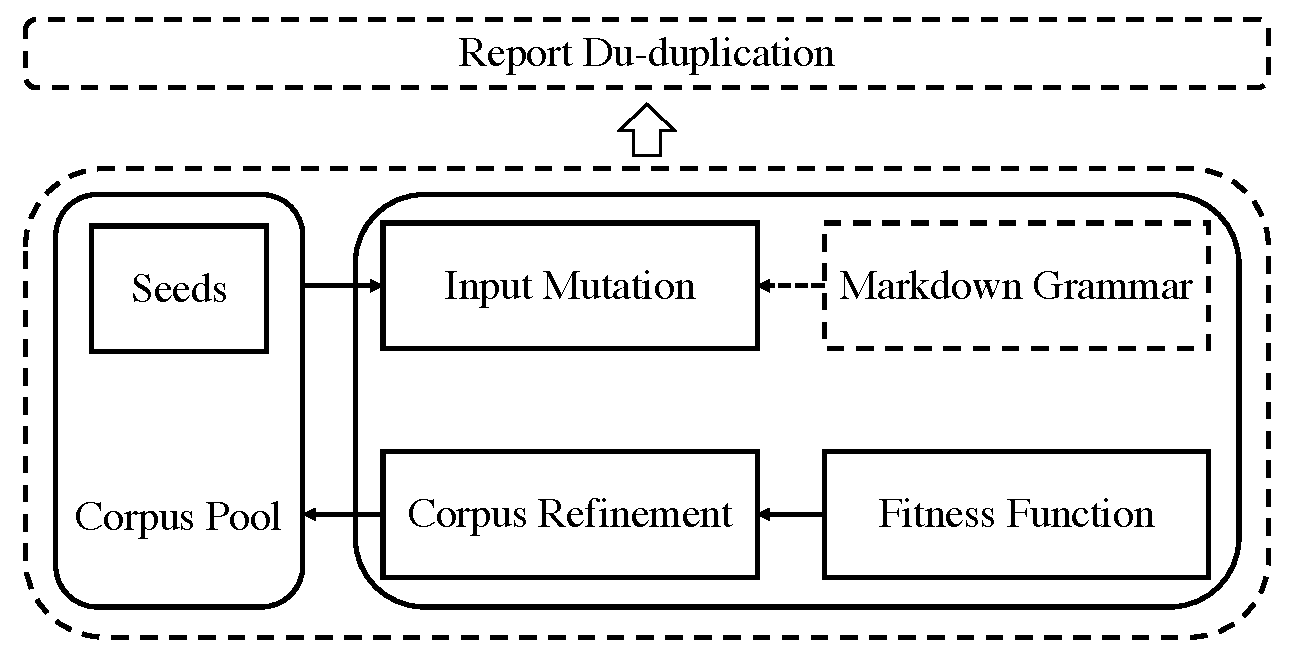
\includegraphics[width=0.45\textwidth]{fig/ase-parser-dos.pdf}
    \caption{The architecture of \sys.
    }
    \label{fig:arch}
\end{figure}

Though we have characterized known performance bugs, %in \autoref{s:study},
%
it is unclear if there exist many unknown performance bugs in the network operating systems.
%
Therefore, we try to detect performance bugs in real-world network operating systems.
%
We focus on CPU resource exhaustion performance bugs in this work because they are the dominant type of performance bugs.
%Due to the high false positives and the excessive manual efforts required in static analysis \cite{rathnayake2014static, wustholz2017static},
%
%dynamic methods are usually preferred.
%

To avoid the high false-positive rates in static analyses \cite{nistor2013toddler,nistor2015caramel},
%
we propose to use dynamic fuzz testing to detect and exploit performance bugs.
%aiming to eliminate the false-positive reports.
%
%Similar to existing works in ReDoS \cite{freezing},
%we also leverage a black-box dynamic testing method to detect performance bugs.
%
%
%The main idea behind our methodology is to leverage test cases to dynamically test real-world applications and platforms and check whether they are vulnerable to performance bugs.
%
To do so, we face a technical challenge.
%
Since many distinct inputs can trigger the same performance bug, it is naturally challenging to accurately de-duplicate the bug reports.
%
Prior performance bug fuzzers \cite{slowfuzz, hotfuzz} do not try to de-duplicate performance bugs.
%
Other fuzzers for detecting \emph{memory corruptions} de-duplicate bugs using the unique memory footprints (\eg{,} coverage profiles and call stacks \cite{klees2018evaluating}) when the bugs are triggered,
%
whereas one \emph{performance bug} can potentially exhibit different memory footprints.
%distinguish abnormal program behaviors from normal ones.
%
%Third, diverse implementations in different programming languages make the bug detection task even harder.
%
%Developing a language-agnostic solution is hard.

%\subsection{Overview}
We overcome these challenges with \sys.
%
The overall methodology is depicted in \autoref{fig:arch}.
%
\sys follows the general fuzzing workflow and is built on top of AFL \cite{afl}.
%
Inside the main fuzzing loop, 
%
to guide the fuzzer to detect CPU resource exhaustion performance bugs,
we use a fitness function to measure if an input should be favored or not
%
(\autoref{s:method-fitness-function}).
%
The fitness function considers both code coverage and resource usage.
%
To report only unique bugs, we transform the execution trace of each report into a vector.
%
We compute the cosine similarity of vector (report) pairs and group highly similar reports as duplicate ones (\autoref{s:method-de-duplicating}).
%
We then present the implementation details (\autoref{s:method-impl}).

\subsection{Fitness Function and Performance Bug Detection}
\label{s:method-fitness-function}
\sys uses a fitness function to decide whether to favor a test case or not.
%
%Coverage-based fitness function enables the fuzzers to explore more new code locations.
%
%
We include both the coverage and the control flow graph (CFG) edge hits into the fitness function.
%
As in other works \cite{oss-fuzz, peng2018tfuzz, klees2018evaluating}, the coverage feedback drives \sys to explore more newly discovered code.
%
Only it, however, is not sufficient for our purpose as it does not consider loop iterations which are crucial for detecting high-complexity performance bugs \cite{slowfuzz}.
%
The CFG edge hits, standing for the times a CFG edge is visited under a test case, enables \sys to explore \emph{computationally expensive} paths.
%
As stated in prior work \cite{perffuzz}, many programs (\eg{,} PHP hash functions \cite{perffuzz, php-hash}) do have non-convex performance space.
%
We thus do not use the execution path length (\eg{,} number of executed instructions) to guide \sys because it might fail to find the performance issues caused by local maxima.
%to the ability to overcome local maxima in a non-convex performance space
%
Therefore, as in the state-of-the-art work, PerfFuzz \cite{perffuzz}, we design \sys to favor those test cases that maximize certain CFG edges to better detect performance bugs.
%
In this way, \sys tends to select test cases to either trigger new code or exhaust certain CFG edges.
%
Note that we do not use runtime CPU usage or concrete execution time as the metric,
%
because they show large variations affected by many uncontrollable factors, such as fuzzer's concurrent features and the characteristics of testing applications.

\iffalse
%With the fitness function, \sys favors several cases that maximize at least one CFG edge during fuzzing.
As stated in \cite{hotfuzz}, an explicit definition of performance bugs of a testing program relies on domain knowledge and manual analysis.
%
This is realistic and pragmatic because it is necessary to understand intended resource consumption bounds.
%
%Not all these test cases necessarily trigger performance bugs as their overall performance slowdown might be light.
%
%
Therefore,
%
we evaluate the test cases to obtain their execution path lengths.
%
We configure a resource computation threshold and label those cases that exceed it as performance bugs.
\fi
%
%

We design a statistical model to accurately identify performance bugs.
Our statistical model first obtains the normal program execution behaviors to label abnormal ones as performance bugs.
%
In particular, though the fitness function favors the local maxima, we still consider the total execution path length as the criteria of performance bugs.
%
The execution path length is calculated as the sum of the CFG edge hits under a test case.
%
We first prepare abundant random normal test cases;
%
we feed each test case to the testing program and obtain the corresponding execution path length.
%
We calculate the the mean ($l_{\mu}$) and the standard deviation ($l_{\sigma}$) of the execution path lengths ($l_i$).
%
We label a case as a performance bug if its execution path exceeds the normal level to a certain extent.
%
%as in Rampart \cite{rampart}, a defense against sophisticated CPU-exhaustion DoS attacks,
%
According to Chebyshev inequality (as shown in \autoref{chebyshev}),
%can measure the probability that one observation differs from the mean of the samples.
%
the probability of the random variable $l_{i}$ that is k-standard deviations away from the mean ($l_{\mu}$) is no more than ${1}/{k^2}$.
%
%Even though we enforce that all test cases are in the size of $m$, we do not assume any underlying distributions of the random variable $T_{r}$ on the uses of Chebyshev inequality.
Since only in rare cases would the execution path length significantly deviate from the normal situations,
%
therefore, we label a performance bug if its execution path length $l_{t}$ is more than $kl_{\sigma}$ away from the $l_{\mu}$ (see \autoref{label}).
%
%
%
%We configure a maximum threshold for a high detection efficiency because some attack inputs may take several hours to process.

\begin{equation} \label{chebyshev}
    P(|l_{i}-l_{\mu}| > k l_{\sigma}) \leq \frac{1}{k^2}
\end{equation}

\begin{equation} \label{label}
    l_{t} > l_{\mu} + kl_{\sigma}
\end{equation}

\subsection{Report De-Duplication}
\label{s:method-de-duplicating}

Though different test cases could all exceed the threshold, they could actually trigger the same performance bug.
%
De-duplicating the bug reports is necessary for a more precise result,
whereas prior works \cite{slowfuzz, perffuzz} do not apply automated methods to de-duplicate the reports.
%
Existing fuzzing works identify unique bugs using the call stack for memory corruptions (\eg{,} crashes).
%
However, it does not fit well our purposes for performance bug de-duplication.
%
Though we can possibly collect the call stack as well (\eg{,} by forcibly terminating the program at some point), the call stack might not be accurate enough to differentiate unique bugs.
%
This is because the exactly critical call stack for a performance bug can hardly be accurately exposed.
%
Unlike memory corruptions that have a deterministic call stack when a bug is triggered,
performance bugs might exhibit diverse call stacks depending on when to obtain them.
%
Therefore, a better report de-duplication method is needed.

We propose a new bug de-duplicating approach by merging reports with similar execution traces.
%
The high-level idea is that different exploiting inputs of the same performance bug should exhibit similar execution traces, \ie{,} most CFG edges are visited in similar frequencies.
%
In particular, we apply the test cases in the reports to the instrumented target software and obtain the CFG edge hits for each edge.
%
We summarize the unique CFG edges that are visited in all reports during fuzz testing into an $n$-dimensional vector space, where $n$ is the total number of unique CFG edges being visited and each dimension in the vector space corresponds to a CFG edge.
%
For each report, we construct an edge-hit vector, \eg{,} $\vv{v}=\left (c_1, c_2, ... , c_n \right )$.
%
Each dimension ($c_i$) represents the hit count of the $i$th CFG edge in that report.
%is the CFG edge hits, which is a non-negative value, \ie{,} $c_i \geq 0$.
%
%$c_i$ is 0 only when the corresponding CFG edge is not visited in the execution trace of the report.
%
To consider if two reports point to the same bug, we construct their edge-hit vectors (\eg{,} $\vv{v}, \vv{v}'$) and compute the cosine similarity (as shown in \autoref{sim}).
%\WM{Do two vectors always have the same number of unique edges? How do you order the edges in the vector?}
%
Cosine similarity is based on the inner product of the two vectors and thus naturally assigns higher weights to the dimensions with larger values (\ie{,} edges visited most).
%
%When triggering a performance bug, certain CFG edges are usually visited more than the others \ie{,} hot edges.
%
Therefore, we calculate the cosine similarity between every two reports and merge reports as the same bug if the cosine similarity of their corresponding edge-hit vectors exceeds a threshold.
%
%We believe it can accurately measure the similarity of the two reports.

\begin{equation} \label{sim}
    Sim(\vv{v}, \vv{v}') = \frac{\vv{v}\cdot \vv{v}'}{|\vv{v}||\vv{v}'|}\
    = \frac{\sum_{j=1}^{n}{c_jc_j'}}{\sqrt{\sum_{j=1}^{n}{c_j^2}} \sqrt{\sum_{j=1}^{n}{c_j'^2}} }
\end{equation}

%
\iffalse
We take a two-step matching approach to efficiently de-duplicate reports.
%
%the simplest algorithm is to compute the cosine similarity of every two reports.
%a program usually contains over 10K distinct CFG edges thus the vector space has over 10K dimensions correspondingly;
%Since
%
%The time complexity of calculating the cosine complexity of two $n$-demensional vectors is roughly $O(n)$ as each dimension is computed for a constant time.
%
%Therefore, the time complexity of the simple algorithm is $O(n \cdot m^2)$, where $m$ is the total number of reports.
%
%However,
%it is very expensive to perform cosine similarity calculation for such an algorithm time complexity because the edge vector space usually has large dimensions (\ie{,} $m >> n$).
%
%
%fuzzing usually produces about 1K reports.
%
%
%\WM{The description was not that clear.}
%\WM{You reduce the vector size like you downsample images, from 100 dimensions into 10 dimensions of which each one is the average value of the previously adjacent 10 dimensions. Then you still do a pair-wise comparison but it would be much more efficient. Then the similar ones are grouped into a cluster.}
First, 
since the edge vector space is usually large, \eg{,} $n > 10,000$,
we reduce the size of the edge vector space by merging a few (\eg{,} 100) adjacent dimensions into one dimension taking their average value.
%
The reduced vector serves as a rough signature of a report.
%
We then compute the cosine similarity of every two reduced vectors and group similar reports into buckets in a coarse-grained manner.
%
%Note that this is more efficient than calculating the exact cosine similarity of original vectors as the vector space size is hugely reduced.
%
%Specifically, we use a relatively lower threshold to cluster the reports into several buckets.
%
Second, within each bucket of similar reports, we compute the exact cosine similarity between two original vectors (reports), classify highly similar ones as a distinct bug.
%
In this way, compared to calculating the exact cosine similarity between every two reports, the time complexity can potentially be reduced by several orders of magnitude.
%
%We will discuss the threshold $sim_t$ later in \autoref{s:eval-parameter}
%
%We configure a maximum threshold for a high detection efficiency because some attack inputs may take several hours to process.
\fi

%

\subsection{Implementation}
\label{s:method-impl}
We implemented the fuzzing part of \sys above an AFL-based fuzzer, PerfFuzz \cite{perffuzz}.
%
Specifically,
we enhanced a C/C++ compiler to instrument the testing software;
we modified AFL's \cc{showmap} functionality to trace the execution on the instrumented applications to obtain the CFG edge hits for report de-duplication.
%
%We implemented our report de-duplicating part with 500 lines of Python code.



\iffalse
\subsection{Performance Bug Detection}
\label{s:method-model}
We build a statistical model to accurately distinguish the normal behaviors and abnormal ones for detecting performance bugs.
%
%\ZMX{A statistical model for what?}
%
As discussed before, using execution time is a common practice in identifying performance bugs \cite{rampart, freezing},
%\ZMX{Exeuction time is not a practice.}
%
so we also use it in our statistical model.
%
%
Our statistical model requires a training stage by feeding the program with $N_r$ random test cases ($I_{r}$) and obtaining the corresponding execution time ($T_{r}$).
%
To eliminate the impacts of the input sizes,
%
we require all the test cases used in our statistical model to be in a constant size, $m$.
%
%Based on basic statistic analysis,
%Statistically, we can regard the execution time as a random variable.
%\ZMX{$T_{r}$ is the set of execution time on a set of test cases. Why can it be a random ``variable''?}
%
We compute the mean ($T_{\mu}$) and the standard deviation ($T_{\sigma}$) of the $N_r$ execution times ($T_{r}$),
%
%Thus its probability distribution can roughly belong to normal distributions.

Our statistical model requires a training stage by feeding the program with $N_r$ random test cases ($I_{r}$) and obtaining the corresponding execution time ($T_{r}$).
%
To eliminate the impacts of the input sizes,
%
we require all the test cases used in our statistical model to be in a constant size, $m$.
%
%Based on basic statistic analysis,
%Statistically, we can regard the execution time as a random variable.
%\ZMX{$T_{r}$ is the set of execution time on a set of test cases. Why can it be a random ``variable''?}
%
We compute the mean ($T_{\mu}$) and the standard deviation ($T_{\sigma}$) of the $N_r$ execution times ($T_{r}$),
To identify performance bugs that could cause spend the underlying network operating systems an extremely long execution time,
%
%as in Rampart \cite{rampart}, a defense against sophisticated CPU-exhaustion DoS attacks,
%
as in \cite{rampart}, we also use the Chebyshev inequality (as shown in \autoref{equ1}) to measure the probability that one observation differs from the mean of the samples.
%
Specifically, the probability of the random variable $T_{r}$ that is k-standard deviations away from the mean ($T_{\mu}$) is no more than ${1}/{k^2}$.
%
Even though we enforce that all test cases are in the size of $m$, we do not assume any underlying distributions of the random variable $T_{r}$ on the uses of Chebyshev inequality.
%
Therefore, in the testing stage, we use \autoref{equ2} to label a performance bug if its execution time on a test case $T_{test}$ is more than $kT_{\sigma}$ away from the mean ($T_{\mu}$) or reaches the maximum time threshold ($T_{max}$).
%
We configure a maximum threshold for a high detection efficiency because some attack inputs may take several hours to process.

\begin{equation} \label{equ1}
    P(|T_{r}-T_{\mu}| > kT_{\sigma}) \leq \frac{1}{k^2}
\end{equation}

\begin{equation} \label{equ2}
    T_{test} > min(T_{\mu} + kT_{\sigma}, T_{max})
\end{equation}
\fi

%\input{impl}
%\section{Detecting Performance Bugs via \sys}
\label{s:eval}
In this section, we investigate the prevalence of performance bugs in the wild.
%
We planed to test network operating systems via fuzzing in this work.
%
However, we temporarily failed to do so due to some practical issues.
%
For example, 1) the time for this research project is too short;
%
and 2) we have not found a flexibile way to apply our instrumented C/C++ compilers to compile an executable network operating systems for the fuzzing.
%
After more than one week exploration, we decided to give it up.
%
Give the truth, we apply \sys to detect performance bugs in othe systems.
%
Since the methodology we propose in this work is general thus we test \sys in 3 compilers\footnote{The authors choose them as they have worked on related topics before.} to verify its efficacy.
%
We naturally admit this limitation.
%
However, we still believe this engineering problem can be fixed give more time.
%
We will definitely make it as our future work.


\PP{Experiments}
Each compiler is first instrumented using our enhanced C compiler in \sys.
%\WM{Where did you introduce this enhanced C compiler? What kind of instrumentation is performed?}
%
We then apply \sys to detect performance bugs on the instrumented compilers.
%
%
We apply the PoCs collected in \autoref{s:study} as the initial seeds
%
and configure \sys to use a single process and a timeout of 6 hours.
%
Through our preliminary study, we empirically set $k$ to 5 and the cosine similarity threshold to 0.91 for all testing software.
%
All experiments described in this section are conducted on a server running Debian GNU/Linux 9, with an Intel Xeon CPU and 96GB RAM.
%\WM{What is the resource computation threshold you use in the evaluation?}
%\PENGHUI{we empirically set that.}
%
%We run the experiments of each process all in a single process.
%We use the Linux \cc{time} command to measure the execution time of a program executed in a single process.
%
%Specifically, we measure the CPU time spent in both user-mode code and kernel.
%

%
%For each test, we use a single process to escape some multiple-process optimizations.
%
%
%For each pattern, we try to repeat the attacking core and insert necessary redundant content.
%
%
\subsection{Results}

\begin{table}[t]
\centering
\caption{The dataset of the compilers and bug detection results.
Rep. is the reports from the fuzzer.
U-Rep. is the unique report after de-duplicating the reports.
Con. means the confirmed bugs.
%Pop. denotes the popularity described using the number of stars and forks of the repositories on the code hosting websites.
    }
\label{table:eval-compiler}
\small
%\resizebox{0.47\textwidth}{!}{
\begin{tabular}{lccccc}
   \toprule
    Software & Lang. & \# Rep. & \# U-Rep. \\
    \midrule
    cmark (0.29.0) &C & 1321 & 7  \\
    MD4C (0.4.7) & C & 239 & 3  \\ 
    cmark-gfm (0.29.0) & C & 981 & 4 \\
    \bottomrule
\end{tabular}
%}
\end{table}




%\input{table}

%
%
We present the performance bug detection results in \autoref{table:eval-compiler}.
%
Duplicate performance bug reports are naturally common during fuzzing.
%
The fuzzing part of \sys reported \num{2541} cases in total and our de-duplicating algorithm merged them into 14 distinct reports.
%
We observe that all the 14 cases did successfully slow down the compilers by 2.31\x to 7.28\x compared to normal-performance cases.
%\WM{How slow?}
%

We further manually check the reports to validate the performance bugs.
%
Since \sys limits the input size like in other works \cite{oss-fuzz, slowfuzz, perffuzz} due to the concerns of large search space, 
%
our manual analysis attempts to identify the severity of the performance slowdown in more realistic scenarios, \ie{,} larger input sizes.
%
To this end, we first identify the exploit input patterns in the reports that exhaust the run-time resources.
%
With the patterns, we further construct larger test cases to verify the performance issues in practice.
%
Finally, 7 cases in 2 compilers were confirmed as performance bugs, including 4 new bugs, after our manual analysis.
%
We are in the process of reporting the new bugs to the concerned vendors.
At the time of writing, 1 bug has been well acknowledged.

We found no bug in MD4C.
%
The developers of MD4C explicitly mention that they seriously considered the performance as one of their main focuses during the implementation \cite{md4c}.
%
%Therefore, such a difference among compilers might suggest that the efforts devoted to the performance issues were different among the different compilers' developers. 
Therefore, the performance bugs could be avoided with domain knowledge and special care, which are often difficult for most developers.
%
%We will discuss the false-positive cases in \autoref{s:eval-fp}.
%

%\subsubsection{False Positives}
%\label{s:eval-fp}
%As presented in \autoref{table:eval-compiler}, \sys has false positives.

\subsection{Comparison}
\label{s:comparison}
We compare \sys with two state-of-the-art works, SlowFuzz \cite{slowfuzz} and PerfFuzz \cite{perffuzz}.
%
\sys and PerfFuzz are implemented above AFL whereas SlowFuzz is built on top of libFuzzer \cite{libfuzzer}.
%
SlowFuzz (libFuzzer) uses in-process fuzzing, which is much faster as it has no overhead for process start-up; however, it is also more fragile and more restrictive because it traps and stops at crashes \cite{libfuzzer}.
%\WM{You write one sentence not two with one period.}
%
Nevertheless, 
we evaluate all the tools with the same dataset in \autoref{table:eval-compiler} and run them for the same amount of time---6 hours---for a fair comparison.
%
We failed to run SlowFuzz on MD4C because of some unexpected crashes after several minutes of the execution.
%
To the best of our knowledge, there is no way to suppress such crashes.
%
\sys and PerfFuzz---AFL-based fuzzers---do not suffer from this problem.
%

The results show that \sys outperformed PerfFuzz and SlowFuzz by detecting more performance bugs.
%
In particular, PerfFuzz reported 820/114/783 cases in cmark/MD4C/cmark-gfm, respectively;
%
SlowFuzz reported 432/408 cases in cmark/cmark-gfm, respectively.
%
These results also demonstrate the need of a report de-duplication method.
%
We applied our report de-duplication algorithm to identify unique bugs and then manually confirmed the reports.
%
Finally, PerfFuzz detected 2/0/2 real performance bugs in cmark/MD4C/cmark-gfm, respectively.
%
SlowFuzz detected 1/1 real performance bugs in cmark/cmark-gfm, respectively.

%Next, we further study the performance slowdown caused by each tool and its code coverage.

\subsubsection{Performance Slowdown}
\label{s:eval-slowdown}

\begin{table}[t]
\centering
    \caption{The performance slowdown and code coverage of \sys, PerfFuzz \cite{perffuzz}, and SlowFuzz \cite{slowfuzz}.
    The Best Slowdown across all tools is normalized over the baseline of the same random normal-performance case.
    Line Cov. and Func. Cov. denote line coverage and function coverage, respectively.
    }
\label{table:eval-comparison}
\small
%\resizebox{0.47\textwidth}{!}{
    \begin{tabular}{clccc}
        \toprule
        Tool & Software & Best Slowdown & Line Cov. & Func. Cov. \\
        \midrule
        \multirow{3}{*}{\rotatebox[origin=c]{90}{\tiny{\sys}}} \
        & cmark & 7.28\x & 71.90\% & 67.91\%\\
        & MD4C & 2.31\x & 76.22\% & 58.11\%\\
        & cmark-gfm & 6.54\x & 55.78\% & 57.35\%\\
        \midrule
        \multirow{3}{*}{\rotatebox[origin=c]{90}{\tiny{ PerfFuzz}}} \
        & cmark & 6.82\x & 56.21\% & 51.35\%\\
        & MD4C & 2.21\x & 67.20\% & 50.20\%\\
        & cmark-gfm & 5.05\x & 48.26\% & 44.31\%\\
        \midrule
        %\multirow{2}{*}{\rotatebox[origin=c]{60}{\scriptsize{SlowFuzz}}} & cmark \\
        \multirow{2}{*}{\rotatebox[origin=c]{90}{\tiny{SlowFuzz}}} \
        & cmark & 4.32\x & 40.28\% & 41.65\%\\
        & cmark-gfm & 3.29\x & 38.30\% & 42.33\%\\
        \bottomrule
    \end{tabular}
%}
\end{table}

\autoref{table:eval-comparison} shows the performance slowdown caused by the inputs generated by \sys, PerfFuzz, and SlowFuzz.
%
We use the maximum execution path length as the performance metric, 
%
%As suggested in \cite{perffuzz}, we also use the sum of CFG edge hits under a test case as the execution path length.
%
%\WM{In your design, you argued that this is not a good metric so you used a different one.}
%
and normalize the performance slowdown using a baseline of a random normal-performance case.
%
We notice that, though all tools caused performance slowdown on the testing applications,
%
\sys achieved a 14.71\% higher average best performance slowdown over PerfFuzz, and 41.21\% over SlowFuzz.
%
Furthermore, we observe that \sys could generate inputs that slow down the compilers much faster than the other tools.
%
For example, to reach a 4.32\x performance slowdown on cmark,
\sys took 3.2 hours, whereas PerfFuzz and SlowFuzz used 3.9 hours and 6.0 hours, respectively.
%
This demonstrates the high efficacy of \sys in detecting performance bugs.

\subsubsection{Code Coverage}
%
We also evaluate the code coverage each tool achieves.
%
We collect the test cases generated by each tool and run on afl-cov \cite{afl-cov},
%
which detects the code coverage using the overall execution traces covered by the test cases.
%
Though SlowFuzz is not based on AFL, we believe using its test cases on afl-cov can accurately reflect the code coverage under a fair metric.
%

We present the results of line coverage and function coverage in \autoref{table:eval-comparison}.
%
\sys outperformed PerfFuzz by 20.75\% more lines of code and 13.17\% more functions;
%
\sys outperformed SlowFuzz by 28.68\% more lines of code and 19.80\% more functions.
%

%\input{eval-other}
%\input{eval-char}
\section{Limitations}
This work has several limitations that need to be further addressed.
%
First, we failed to instrument some network operating systems for the evaluation and alternatively evaluated in other systems.
%
This problem, was out of the foreseeable scope of the authors when proposing the idea.
%
The authors also were not able to fix it given limited time.
%
Though our technique is general, there might be some unknown challenges that we cannot foresee now.
%
We have to tackle this limitation to make \sys applicable for our initial purposes.
%
Nevertheless, our evaluation somehow demonstrated the efficacy of \sys.
%
Similarly, we are in certain confidence that \sys can also perform excellently once the above challenge is solved. 
%
Second, also due to the lack of human efforts, the empirical study is deep enough.
%
There are many other interesting aspects that can be studied further.
%
For example, how are the performance bugs patched?
%
We will further investigate these directions in the future.


%\section{Related work}
\label{s:relwk}

\PP{Understanding performance bugs}
Understanding the characteristics of performance bugs can help design techniques to detect and fix performance bugs.
%
Existing studies focus on the performance bugs in programs on the desktop platform \cite{perfbugstudy, zaman2012qualitative}, mobile platform \cite{liu2014characterizing}, and the web server end \cite{perfbugstudy}, \etc{}
%
For instance, Zaman \etal{} studied performance bugs in Firefox and Chrome and provided suggestions to fix the bugs and to validate the patches \cite{zaman2012qualitative}.
%
However, there is little understanding of performance bugs in the network operating systems.
%
Sub \etal{} studied GCC and LLVM compilers but they did not focus on the performance issues \cite{sun2016toward}.
%
Our work studies an understudied problem---performance bugs.

\PP{Detecting performance bugs}
The detection of performance issues has drawn significant attention from researchers over the past years.
%
Prior studies focus on application-layer DoS vulnerabilities \cite{rampart, jazi2017detecting, durcekova2012sophisticated}, 
%
algorithmic complexity DoS vulnerabilities \cite{crosby2003algodos, smith2006backtracking}, and other general performance issues \cite{perfbugstudy,liu2014characterizing}.
%that exhaust CPU resources.
Static methods analyze the source code of the applications and diagnose vulnerable bug patterns, for example, repeated loops \cite{nistor2013toddler,nistor2015caramel}.
%
Dynamic methods are also applied to identify performance bugs.
%
SlowFuzz \cite{slowfuzz}, PerfFuzz \cite{perffuzz}, and HotFuzz \cite{hotfuzz} propose new fuzzing solutions to detect the worst-case algorithmic complexity vulnerabilities.
%
%Hybrid approaches \cite{shen2018rescue} combine static analysis and dynamic test generation to detect performance bugs like ReDoS problems in the Java engine.
%
Our work improves existing solutions via a fitness function and a new report de-duplication method.
%
Our evaluation has well demonstrated its efficacy.
%

\section{Conclusion}
\label{s:conclusion}
Performance bugs in network operating systems are previously understudied.
%
This paper conducted a systematic study to understand the characteristics of the performance bugs.
We designed \sys with several new techniques to detect performance bugs in the wild.
%
Our evaluation demonstrates report de-duplication is necessary and our solution is effective.
%
We hope our research, as an initial step, can shed some light on future security analysis and software developments.

%\section*{Acknowledgment}
\label{s:ack}
The authors would like to thank the anonymous reviewers for their helpful suggestions and comments.
The work described in this paper was mainly supported by a grant from the Research Grants Council of the Hong Kong Special Administrative Region, China (Project No. CUHK 14210219).


%\balance
%\interlinepenalty=10000
\bibliographystyle{ACM-Reference-Format}
%\footnotesize
%\setlength{\bibsep}{3pt}
\bibliography{p,conf}
\begin{appendices}
\section{CVEs in Our Study}
\label{cve-details}

\section{Future Work}

\section{Artifact Instructions}

\end{appendices}


%%%%%%%%%%%%%%%%%%%%%%%%%%%%%%%%%%%%%%%%%%%%%%%%%%%%%%%%%%%%%%%%%%%%%%%%%%%%%%%%
\end{document}
%%%%%%%%%%%%%%%%%%%%%%%%%%%%%%%%%%%%%%%%%%%%%%%%%%%%%%%%%%%%%%%%%%%%%%%%%%%%%%%%

%%  LocalWords:  endnotes includegraphics fread ptr nobj noindent
%%  LocalWords:  pdflatex acks
